\chapter{ठोस-अवस्था रसायन: बैंड, दोष और अर्धचालक}\label{ch:b3:solid-state}

छत पर लगा सौर पैनल और लैंप का प्रकाश-उत्सर्जक डायोड एक ही प्रकार के क्रिस्टल से बने हैं,
सिलिकॉन या नाइट्रोजन, आर्सेनिक या फ़ॉस्फ़ोरस के साथ गैलियम का कोई यौगिक, जिसमें
जानबूझकर प्रति दस लाख कुछ अशुद्धि परमाणु डाले गए हैं। उनकी कार्यप्रणाली दो ऐसी चीज़ों से
तय होती है जो किसी अणु में नहीं होतीं: ऊर्जा स्तरों के बैंड, एक अंतराल सहित जिसकी चौड़ाई
तय करती है कि क्रिस्टल कौन-सा प्रकाश अवशोषित या उत्सर्जित करता है, और दोष, जो आवेश वहन करते हैं। यह अध्याय
आण्विक कक्षकों से बैंड बनाता है, किसी \omterm{def:b3:solid-state:classes}{अर्धचालक} के वाहकों की गिनती करता है, और
लुप्त तथा गलत स्थान पर स्थित परमाणुओं को अपने साम्यों वाली रासायनिक स्पीशीज़ के रूप में देखता है,
कार के निकास में लगे ऑक्सीजन संवेदक के \omterm{def:b3:solid-state:ionic-conductor}{ठोस विद्युत-अपघट्य} तक।

\begin{recall}
प्रथम वर्ष के खंड ने क्रिस्टल, धात्विक आबंध, आयनिक और सहसंयोजी
क्रिस्टल, अंतराकाशी स्थल और मिश्रधातुएँ, तथा नेर्न्स्ट समीकरण परिभाषित किए; द्वितीय वर्ष के
खंड ने ह्युकेल विधि और अनुनाद समाकल $\beta$।
\Cref{ch:b3:x-ray-diffraction} ने \omterm{def:b3:x-ray-diffraction:reciprocal}{व्युत्क्रम जालक} दिया और
\cref{ch:b3:partition-functions} ने \omterm{def:b3:partition-functions:boltzmann}{बोल्ट्समान वितरण} और
\omterm{def:b3:partition-functions:statistical-entropy}{सांख्यिकीय एन्ट्रॉपी} $S = k\ln W$।
\end{recall}

\begin{omfigure}
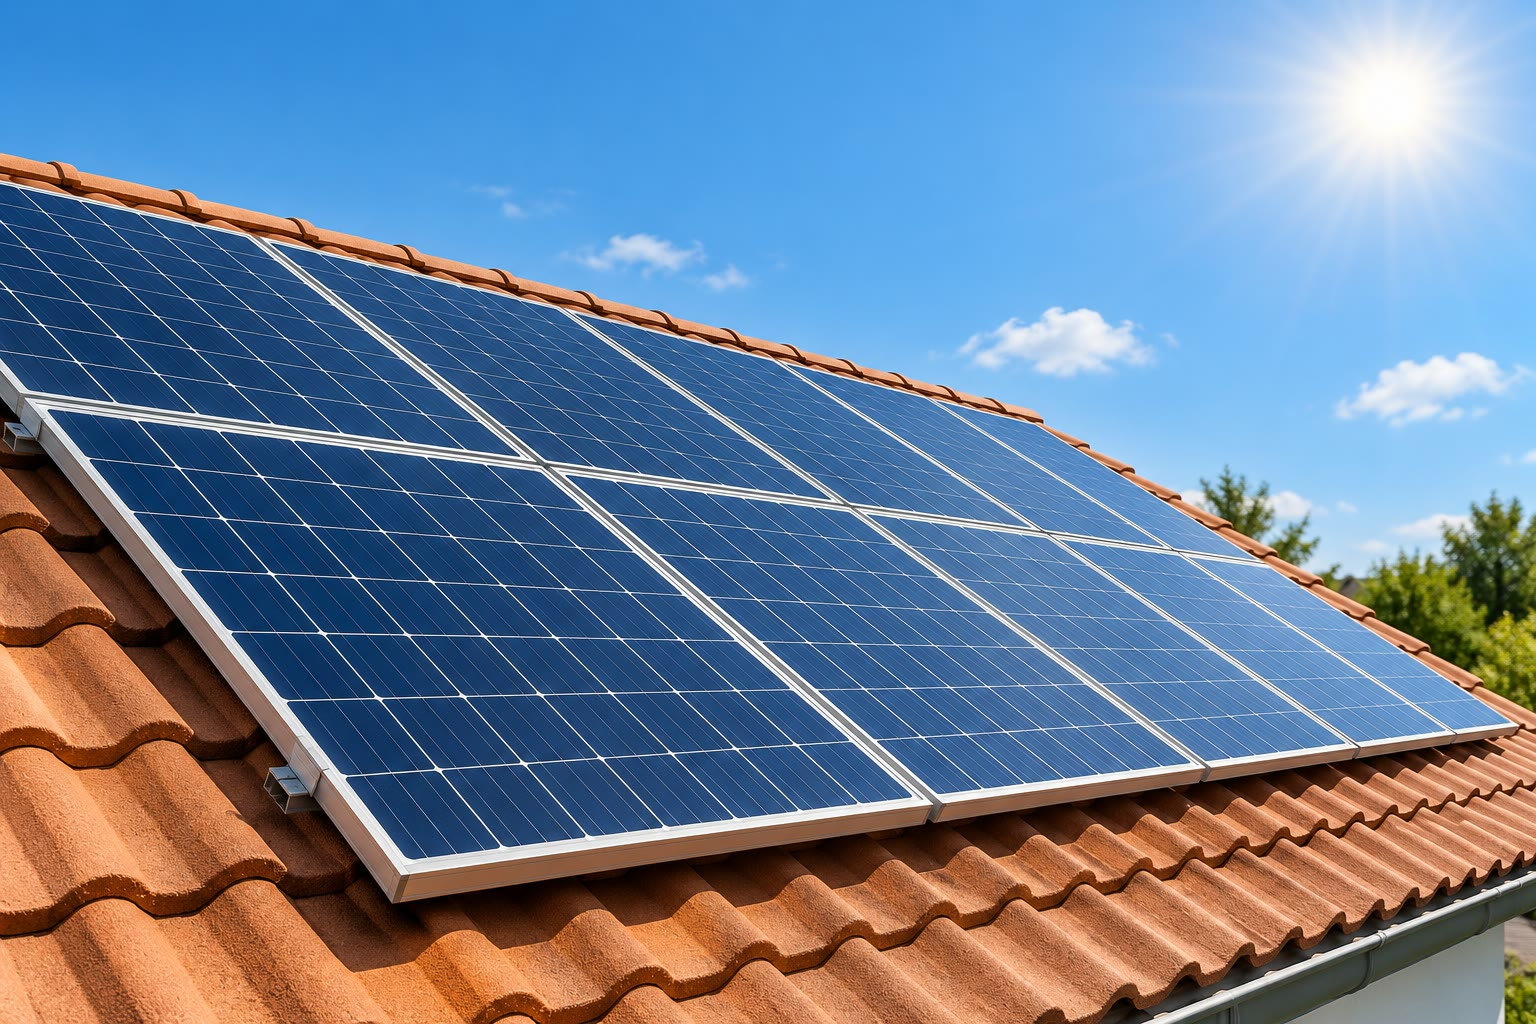
\includegraphics[width=0.6\linewidth]{images/book4/ai/b3-22-solar-panels.jpg}

{\small खपरैल की छत पर सौर पैनल: प्रत्येक सेल सिलिकॉन की एक पतली परत है, जिसमें
प्रकाश इलेक्ट्रॉनों को लगभग एक इलेक्ट्रॉनवोल्ट के \omterm{def:b3:solid-state:band}{बैंड अंतराल} के पार उठा देता है।}
\end{omfigure}

\section{कक्षकों से बैंडों तक}

ह्युकेल सन्निकटन में $N$ सर्वसम परमाणुओं की एक शृंखला लीजिए, जिनमें से प्रत्येक में एक s कक्षक हो:
प्रत्येक परमाणु पर कूलॉम समाकल $\alpha$, पड़ोसियों के बीच अनुनाद समाकल $\beta < 0$,
अन्यथा शून्य।

\begin{theorem}[ह्युकेल शृंखला के स्तर]\label{thm:b3:solid-state:chain}
$N$ परमाणुओं की रैखिक शृंखला के $N$ आण्विक कक्षकों की ऊर्जाएँ हैं
\[
  E_k = \alpha + 2\beta\cos\frac{k\pi}{N + 1}, \qquad k = 1, \dots, N,
\]
गुणांकों $c_j^{(k)} \propto \sin\bigl(jk\pi/(N + 1)\bigr)$ के साथ, परमाणु $j$ पर। $N \to \infty$ होने पर स्तर
$\alpha + 2\beta$ से $\alpha - 2\beta$ तक के अंतराल को सघनता से भर देते हैं: चौड़ाई $4|\beta|$ का एक बैंड।
\end{theorem}

\begin{proof}
सेकुलर समीकरण $\beta c_{j-1} + (\alpha - E)c_j + \beta c_{j+1} = 0$ हैं, $j = 1, \dots, N$ के लिए, जहाँ $c_0 = c_{N+1} = 0$
(वहाँ कोई परमाणु नहीं)। $c_j = \sin(j\theta)$ आज़माइए: चूँकि $\sin((j - 1)\theta) + \sin((j + 1)\theta) = 2\cos\theta\sin(j\theta)$, प्रत्येक
समीकरण $(\alpha - E + 2\beta\cos\theta)\sin(j\theta) = 0$ बन जाता है, अतः $E = \alpha + 2\beta\cos\theta$। शर्त $c_0 = 0$
प्रत्येक $\theta$ के लिए सत्य है, और $c_{N+1} = \sin((N + 1)\theta) = 0$ के लिए $\theta = k\pi/(N + 1)$ आवश्यक है; $k = 1, \dots, N$ से $N$ भिन्न
स्तर मिलते हैं (अन्य उन्हें दोहराते हैं या लुप्त हो जाते हैं)। सबसे निचला और सबसे ऊँचा
$\alpha \pm 2\beta\cos(\pi/(N + 1))$ हैं, जो $\alpha \pm 2\beta$ की ओर प्रवृत्त होते हैं; पड़ोसियों के बीच अंतराल अधिक से अधिक
$2|\beta|\pi/(N + 1)$ है, जो शून्य की ओर प्रवृत्त होता है।
\end{proof}

$N = 2$ के लिए प्रमेय $\alpha \pm \beta$ देता है, एथीन के $\pi$ निकाय के कक्षक;
$N = 6$ के लिए विवृत-शृंखला हेक्साट्राइईन। तीन विमाओं में यही हर प्रकार के
परमाण्वीय कक्षक के साथ होता है: s कक्षक एक s बैंड देते हैं, p कक्षक एक p बैंड,
और प्रत्येक बैंड $2N$ इलेक्ट्रॉन रखता है, $N$ परमाणुओं के लिए।

\begin{definition}[बैंड]\label{def:b3:solid-state:band}
किसी क्रिस्टल का \emph{ऊर्जा बैंड}\index{ऊर्जा बैंड} अनुमत एक-इलेक्ट्रॉन
ऊर्जाओं का एक सतत परास है, जो उसके सभी परमाणुओं के कक्षकों से बनता है।
\emph{बैंड अंतराल}\index{बैंड अंतराल} $E_g$ ऊर्जाओं का वह परास है जिसमें दो
बैंडों के बीच कोई स्तर नहीं होता। शून्य ताप पर किसी \omterm{def:b3:solid-state:classes}{अर्धचालक} या \omterm{def:b3:solid-state:classes}{विद्युतरोधी} में सबसे ऊँचा
भरा बैंड \emph{संयोजकता बैंड}\index{संयोजकता बैंड} है और सबसे निचला रिक्त
बैंड \emph{चालन बैंड}\index{चालन बैंड}।
\end{definition}

\begin{definition}[अवस्था घनत्व और फ़र्मी स्तर]\label{def:b3:solid-state:fermi}
\emph{अवस्था घनत्व}\index{अवस्था घनत्व} $g(E)$ ऊर्जा $E$ के निकट प्रति इकाई ऊर्जा
(और प्रति परमाणु या प्रति इकाई आयतन) स्तरों की संख्या है।
\emph{फ़र्मी स्तर}\index{फ़र्मी स्तर} $E_F$ वह ऊर्जा है जिस पर किसी स्तर के अधिकृत होने की
प्रायिकता $1/2$ होती है; शून्य ताप पर इससे नीचे के सभी स्तर
भरे और इसके ऊपर के सभी रिक्त होते हैं।
\end{definition}

\begin{omfigure}
\begin{tikzpicture}
\begin{axis}[width=0.78\linewidth, height=6.2cm, xmin=0.3, xmax=7.6, ymin=-2.3, ymax=2.3,
  axis lines=left, xtick={1,2,3,4,5,6.6}, xticklabels={2,4,8,16,64,$\infty$: $g(E)$},
  xlabel={परमाणुओं की संख्या $N$}, ylabel={$(E - \alpha)/|\beta|$},
  ytick={-2,-1,0,1,2}, tick label style={font=\small}, label style={font=\small}]
\addplot[only marks, mark=-, mark size=7pt, omDef, thick] table[x=col, y=e] {figdata/out/bachelor-3-band-chain.dat};
\addplot[omThm, thick] table[x expr=6.0+0.55*\thisrow{g}, y=e] {figdata/out/bachelor-3-band-chain-b.dat};
\draw[black!40, dashed] (axis cs:0.3,-2) -- (axis cs:7.6,-2);
\draw[black!40, dashed] (axis cs:0.3,2) -- (axis cs:7.6,2);
\draw[<->, black!60] (axis cs:5.6,-2) -- (axis cs:5.6,2) node[midway, left, font=\scriptsize] {$4|\beta|$};
\end{axis}
\end{tikzpicture}

{\small 2 से 64 परमाणुओं की शृंखलाओं के ह्युकेल स्तर (प्रति स्तर एक छोटी रेखा;
$\beta < 0$ के साथ आबंधी स्तर नीचे हैं)। स्तर
$\alpha + 2\beta$ और $\alpha - 2\beta$ के बीच एक बैंड में सिमट जाते हैं; दाईं ओर, अनंत
शृंखला का \omterm{def:b3:solid-state:fermi}{अवस्था घनत्व}, जो बैंड किनारों पर सबसे बड़ा है।}
\end{omfigure}

\begin{proposition}[बैंड का भराव]\label{prop:b3:solid-state:filling}
जिस क्रिस्टल का सबसे ऊँचा अधिकृत बैंड आंशिक रूप से भरा हो, वह धातु की तरह
विद्युत चालन करता है; जिस क्रिस्टल के बैंड या तो पूरे भरे हों या रिक्त, और उनके बीच
एक अंतराल हो, वह शून्य ताप पर चालन नहीं करता।
\end{proposition}

\begin{proof}[तर्क]
विद्युत क्षेत्र में इलेक्ट्रॉन थोड़ी ऊर्जा और संवेग प्राप्त करते हैं: उन्हें
अपने अधिकृत स्तरों के ठीक ऊपर के रिक्त स्तरों में जाना होता है। आंशिक रूप से भरे
बैंड में ऐसे स्तर \omterm{def:b3:solid-state:fermi}{फ़र्मी स्तर} के ठीक ऊपर, बिना ऊर्जा व्यय के, स्थित होते हैं।
पूरे भरे बैंड में हर स्तर अधिकृत है और अगला रिक्त स्तर अंतराल के पार है;
इसके अतिरिक्त, पूरा भरा बैंड कोई नेट धारा वहन नहीं करता, क्योंकि एक दिशा में चलने वाले
प्रत्येक इलेक्ट्रॉन के लिए दूसरा विपरीत दिशा में चलता है।
\end{proof}

सोडियम, प्रति परमाणु एक 3s इलेक्ट्रॉन के साथ, अपना s बैंड आधा भरता है: एक धातु।
मैग्नीशियम, दो के साथ, अपना s बैंड ठीक पूरा भर देता, परंतु s और p बैंड
अतिव्यापित होते हैं, अतः वह भी धातु है। हीरे और सिलिकॉन में प्रति परमाणु चार संयोजकता
इलेक्ट्रॉन ऐसे कक्षकों में होते हैं जो एक भरे आबंधी बैंड और एक रिक्त
प्रतिआबंधी बैंड में विपाटित होते हैं, जो एक अंतराल से पृथक हैं।

\begin{definition}[अर्धचालक और विद्युतरोधी]\label{def:b3:solid-state:classes}
\emph{अर्धचालक}\index{अर्धचालक} वह ठोस है जिसका \omterm{def:b3:solid-state:band}{बैंड अंतराल} इतना छोटा
(लगभग \qty{3}{eV} तक) हो कि सामान्य ताप पर या अपमिश्रण के बाद मापनीय संख्या में इलेक्ट्रॉन
उसे पार कर सकें; \emph{विद्युतरोधी}\index{विद्युतरोधी}
का अंतराल इतना बड़ा होता है कि वह चालन नहीं करता।
\end{definition}

\begin{omfigure}
\begin{tikzpicture}[font=\small]
  \foreach \x/\name in {0/धातु, 3.6/अर्धचालक, 7.2/विद्युतरोधी} {
    \node[font=\small\bfseries] at (\x+0.8,4.3) {\name};
  }
  % metal: one partly filled band
  \fill[omDef!55] (0,0.4) rectangle (1.6,2.0);
  \draw (0,0.4) rectangle (1.6,3.4);
  \draw[omThm, thick] (-0.25,2.0) -- (1.85,2.0) node[right, font=\scriptsize] {$E_F$};
  % semiconductor: small gap
  \fill[omDef!55] (3.6,0.4) rectangle (5.2,1.7);
  \draw (3.6,0.4) rectangle (5.2,1.7);
  \draw (3.6,2.5) rectangle (5.2,3.8);
  \draw[omThm, thick] (3.35,2.1) -- (5.45,2.1) node[right, font=\scriptsize] {$E_F$};
  \draw[<->] (4.4,1.7) -- (4.4,2.5) node[pos=0.8, right, font=\scriptsize] {$E_g$};
  % insulator: large gap
  \fill[omDef!55] (7.2,0.4) rectangle (8.8,1.2);
  \draw (7.2,0.4) rectangle (8.8,1.2);
  \draw (7.2,3.2) rectangle (8.8,4.0);
  \draw[omThm, thick] (6.95,2.2) -- (9.05,2.2) node[right, font=\scriptsize] {$E_F$};
  \draw[<->] (8.0,1.2) -- (8.0,3.2) node[pos=0.75, right, font=\scriptsize] {$E_g$};
  \node[font=\scriptsize, anchor=east] at (3.5,1.05) {संयोजकता};
  \node[font=\scriptsize, anchor=east] at (3.5,3.15) {चालन};
  \draw[->] (-0.6,0.2) -- (-0.6,3.9) node[above, font=\scriptsize] {$E$};
\end{tikzpicture}

{\small शून्य ताप पर बैंड का भराव (भरे स्तर छायांकित)। धातु में
आंशिक रूप से भरा बैंड होता है और उसका \omterm{def:b3:solid-state:fermi}{फ़र्मी स्तर} उसी के भीतर; \omterm{def:b3:solid-state:classes}{अर्धचालक} और
\omterm{def:b3:solid-state:classes}{विद्युतरोधी} में पूरा भरा \omterm{def:b3:solid-state:band}{संयोजकता बैंड} और रिक्त \omterm{def:b3:solid-state:band}{चालन बैंड} होता है, \omterm{def:b3:solid-state:fermi}{फ़र्मी
स्तर} अंतराल में होता है, जो पहले में संकीर्ण और दूसरे में चौड़ा है।}
\end{omfigure}

\section{अर्धचालक}

\begin{definition}[वाहक]\label{def:b3:solid-state:carriers}
\emph{नैज अर्धचालक}\index{नैज अर्धचालक} एक शुद्ध
\omterm{def:b3:solid-state:classes}{अर्धचालक} है, जिसके सभी वाहक अंतराल के पार उत्तेजित इलेक्ट्रॉनों से आते हैं।
\emph{आवेश वाहक}\index{आवेश वाहक} धारा वहन करने वाला एक गतिशील
कण है: \omterm{def:b3:solid-state:band}{चालन बैंड} में एक इलेक्ट्रॉन, या एक \emph{कोटर}\index{कोटर}, अर्थात्
\omterm{def:b3:solid-state:band}{संयोजकता बैंड} में एक रिक्त स्तर, जो धनावेश की तरह गति करता है।
\end{definition}

\begin{theorem}[नैज वाहक सांद्रता]\label{thm:b3:solid-state:intrinsic}
$N_c$ और $N_v$ को चालन और \omterm{def:b3:solid-state:band}{संयोजकता बैंडों} के प्रभावी \omterm{def:b3:solid-state:fermi}{अवस्था घनत्व} (स्वीकृत)
लेने पर, ऐसे \omterm{def:b3:solid-state:classes}{अर्धचालक} की इलेक्ट्रॉन और \omterm{def:b3:solid-state:carriers}{कोटर} सांद्रताएँ,
जिसका \omterm{def:b3:solid-state:fermi}{फ़र्मी स्तर} किसी भी बैंड किनारे से कुछ $kT$ से अधिक दूर हो, ये हैं
\[
  n = N_c\,\eu^{-(E_c - E_F)/kT}, \qquad p = N_v\,\eu^{-(E_F - E_v)/kT},
\]
और \omterm{def:b3:solid-state:carriers}{नैज अर्धचालक} में
\[
  n = p = n_i = \sqrt{N_cN_v}\,\eu^{-E_g/2kT}.
\]
\end{theorem}

\begin{proof}
ऊर्जा $E$ वाले स्तर का अधिभोग $f(E) = 1/(1 + \eu^{(E - E_F)/kT})$ है। जब
$E - E_F \gg kT$, तो $f \approx \eu^{-(E - E_F)/kT}$, एक बोल्ट्समान पुच्छ। \omterm{def:b3:solid-state:band}{चालन
बैंड} के स्तरों पर इसका योग करने पर, $n = \int g_c(E)\eu^{-(E - E_F)/kT}\,\dd E = \eu^{-(E_c - E_F)/kT}\int g_c(E)\eu^{-(E - E_c)/kT}\,\dd E$, और अंतिम समाकल
परिभाषा से $N_c$ है। \omterm{def:b3:solid-state:carriers}{कोटर} रिक्त स्तर हैं, जिनकी प्रायिकता $1 - f \approx \eu^{-(E_F - E)/kT}$
\omterm{def:b3:solid-state:band}{संयोजकता बैंड} में है; वही चरण $p$ देते हैं। तब $np = N_cN_v\eu^{-(E_c - E_v)/kT} = N_cN_v\eu^{-E_g/kT}$, और शुद्ध क्रिस्टल में
प्रत्येक उत्तेजित इलेक्ट्रॉन एक \omterm{def:b3:solid-state:carriers}{कोटर} छोड़ता है: $n = p$, अतः $n = \sqrt{np}$।
\end{proof}

\begin{proposition}[द्रव्य-अनुपाती क्रिया नियम]\label{prop:b3:solid-state:mass-action}
साम्य पर किसी भी \omterm{def:b3:solid-state:classes}{अर्धचालक} में, अपमिश्रित हो या नहीं, $np = n_i^2$।
\end{proposition}

\begin{proof}
\cref{thm:b3:solid-state:intrinsic} की उपपत्ति में प्राप्त गुणनफल $np = N_cN_v\eu^{-E_g/kT}$
में $E_F$ नहीं है: \omterm{def:b3:solid-state:fermi}{फ़र्मी स्तर} को चाहे जो तय करे, यह वही रहता है,
और अपने नैज मान $n_i^2$ के बराबर होता है। यह
$\text{कुछ नहीं} \rightleftharpoons \mathrm e^- + \mathrm h^+$ का साम्य स्थिरांक है, जल के आयनिक गुणनफल की तरह।
\end{proof}

\begin{omfigure}
% ledger: eg:Si.E0, eg:Si.a, eg:Si.b, eg:Ge.E0, eg:Ge.a, eg:Ge.b, dos:Si.Nc, dos:Si.Nv, dos:Ge.Nc, dos:Ge.Nv, dop:Si.P
\begin{tikzpicture}
\begin{axis}[name=a, width=0.45\linewidth, height=5.6cm, xmin=1.2, xmax=4.2, ymin=4, ymax=18,
  axis lines=left, xlabel={$1000\,\mathrm K/T$}, ylabel={$\log_{10}(n_i/\unit{cm^{-3}})$},
  tick label style={font=\scriptsize}, label style={font=\small}]
\addplot[omDef, thick] table[x=invT, y=lgSi] {figdata/out/bachelor-3-semiconductor-carriers.dat};
\addplot[omThm, thick] table[x=invT, y=lgGe] {figdata/out/bachelor-3-semiconductor-carriers.dat};
\node[font=\scriptsize, omDef] at (axis cs:3.4,8.3) {Si};
\node[font=\scriptsize, omThm, anchor=south west] at (axis cs:3.4,14.0) {Ge};
\end{axis}
\begin{axis}[at={(a.east)}, anchor=west, xshift=1.7cm, width=0.45\linewidth, height=5.6cm,
  xmin=1, xmax=25, ymin=10, ymax=17, axis lines=left,
  xlabel={$1000\,\mathrm K/T$}, ylabel={$\log_{10}(n/\unit{cm^{-3}})$},
  tick label style={font=\scriptsize}, label style={font=\small}]
\addplot[omDef, thick] table[x=invT, y=lgn] {figdata/out/bachelor-3-semiconductor-carriers-b.dat};
\addplot[black!45, dashed, unbounded coords=jump, restrict y to domain=10:17] table[x=invT, y=lgni] {figdata/out/bachelor-3-semiconductor-carriers-b.dat};
\node[font=\scriptsize, anchor=west] at (axis cs:2.6,16.4) {नैज};
\node[font=\scriptsize] at (axis cs:12,15.35) {संतृप्ति, $n = N_D$};
\node[font=\scriptsize] at (axis cs:20,13.2) {जमाव};
\end{axis}
\end{tikzpicture}

{\small बाएँ: सिलिकॉन और जर्मेनियम की नैज वाहक सांद्रताएँ,
$1/T$ के विरुद्ध (मापे गए अंतरालों और प्रभावी \omterm{def:b3:solid-state:fermi}{अवस्था घनत्वों} वाला मॉडल); ढलान
$-E_g/2k$ के निकट हैं। दाएँ:
$\qty{1e15}{cm^{-3}}$ फ़ॉस्फ़ोरस से अपमिश्रित सिलिकॉन में इलेक्ट्रॉन: निम्न ताप पर दाता अपने इलेक्ट्रॉन थामे रहते हैं
(जमाव), लगभग 150 से \qty{500}{K} तक सभी आयनित होते हैं ($n = N_D$), और उच्च
ताप पर नैज वाहक (धराशायी, $n_i$) प्रभावी हो जाते हैं।}
\end{omfigure}

\begin{definition}[प्रत्यक्ष और अप्रत्यक्ष अंतराल]\label{def:b3:solid-state:gap-types}
किसी \omterm{def:b3:solid-state:classes}{अर्धचालक} का \emph{प्रत्यक्ष बैंड अंतराल}\index{प्रत्यक्ष बैंड अंतराल} होता है जब
उसके \omterm{def:b3:solid-state:band}{संयोजकता बैंड} का शीर्ष और \omterm{def:b3:solid-state:band}{चालन बैंड} की तली एक ही
इलेक्ट्रॉन संवेग पर हों, जिससे अकेला एक फ़ोटॉन किसी इलेक्ट्रॉन को पार ले जा सके, और
\emph{अप्रत्यक्ष बैंड अंतराल}\index{अप्रत्यक्ष बैंड अंतराल} जब ऐसा न हो, जिससे
संक्रमण के लिए एक जालक कंपन भी आवश्यक हो।
\end{definition}

% ledger: eg:Si, eg:Ge, eg:GaAs, eg:GaN, eg:GaP
सिलिकॉन (\qty{1.12}{eV}) और जर्मेनियम (\qty{0.66}{eV}) के अंतराल अप्रत्यक्ष हैं:
वे मोटी परत में प्रकाश को पर्याप्त अच्छी तरह अवशोषित करते हैं, जो सौर सेल के लिए उपयुक्त है, पर
उसका उत्सर्जन बहुत कम करते हैं। गैलियम आर्सेनाइड (\qty{1.42}{eV}) और गैलियम नाइट्राइड (लगभग
\qty{3.4}{eV}) के अंतराल प्रत्यक्ष हैं, जो अवरक्त और नीले प्रकाश-उत्सर्जक
डायोडों और लेज़रों का आधार हैं; गैलियम फ़ॉस्फ़ाइड (\qty{2.26}{eV}) अप्रत्यक्ष है पर अपमिश्रित होने पर हरा
प्रकाश उत्सर्जित करता है। अनेक वर्णकों का रंग भी एक \omterm{def:b3:solid-state:band}{बैंड अंतराल} है: क्रिस्टल
$h\nu > E_g$ वाले सभी फ़ोटॉन अवशोषित करता है, अतः कैडमियम सल्फ़ाइड, जिसका अंतराल नीले में है,
पीला है।

\begin{definition}[अपमिश्रण]\label{def:b3:solid-state:doping}
\emph{अपमिश्रक}\index{अपमिश्रक} वह बाहरी परमाणु है जिसे वाहक प्रदान करने के लिए
जानबूझकर, कम मात्रा में, किसी \omterm{def:b3:solid-state:classes}{अर्धचालक} में डाला जाता है। \emph{n-प्रकार
अर्धचालक}\index{n-प्रकार अर्धचालक} में अपमिश्रक में, जिस परमाणु का वह स्थान लेता है उससे, एक संयोजकता
इलेक्ट्रॉन अधिक होता है (सिलिकॉन में फ़ॉस्फ़ोरस) और वह उसे उस बैंड के ठीक नीचे स्थित
एक \emph{दाता स्तर}\index{दाता स्तर} से \omterm{def:b3:solid-state:band}{चालन बैंड} को देता है;
\emph{p-प्रकार अर्धचालक}\index{p-प्रकार अर्धचालक} में उसमें एक
कम होता है (सिलिकॉन में बोरॉन) और वह \omterm{def:b3:solid-state:band}{संयोजकता बैंड} से एक इलेक्ट्रॉन को उसके ठीक ऊपर स्थित
एक \emph{ग्राही स्तर}\index{ग्राही स्तर} में ग्रहण करता है, जिससे एक \omterm{def:b3:solid-state:carriers}{कोटर} बचता है।
\end{definition}

\begin{omfigure}
\begin{tikzpicture}[font=\small]
  \foreach \x in {0, 5.2} {
    \fill[omDef!35] (\x,0) rectangle (\x+3.6,1.0);
    \fill[omDef!12] (\x,2.6) rectangle (\x+3.6,3.6);
    \node[font=\scriptsize] at (\x+1.8,0.5) {संयोजकता बैंड};
    \node[font=\scriptsize] at (\x+1.8,3.1) {चालन बैंड};
  }
  \foreach \i in {0,...,5} { \draw[omThm, thick] (0.25+\i*0.55,2.35) -- (0.6+\i*0.55,2.35); }
  \node[font=\scriptsize, anchor=west] at (0.1,1.95) {दाता स्तर, \qty{0.045}{eV} नीचे};
  \draw[->, omThm] (0.42,2.42) -- (0.42,2.9);
  \fill[omThm] (0.42,2.95) circle (1.6pt);
  \foreach \i in {0,...,5} { \draw[omMeth, thick] (5.45+\i*0.55,1.25) -- (5.8+\i*0.55,1.25); }
  \node[font=\scriptsize, anchor=west] at (5.3,1.6) {ग्राही स्तर, \qty{0.045}{eV} ऊपर};
  \draw[->, omMeth] (5.62,0.7) -- (5.62,1.18);
  \draw[omMeth, fill=white] (5.62,0.62) circle (1.8pt);
  \node[font=\small\bfseries] at (1.8,4.0) {n-प्रकार: Si में P};
  \node[font=\small\bfseries] at (7.0,4.0) {p-प्रकार: Si में B};
\end{tikzpicture}

{\small सिलिकॉन के अंतराल में दाता और \omterm{def:b3:solid-state:doping}{ग्राही स्तर} (अंतराल पैमाने पर नहीं:
\omterm{def:b3:solid-state:doping}{अपमिश्रक} स्तर बैंड किनारों से लगभग 0.045 eV पर हैं, अंतराल 1.12 eV है)। एक
दाता अपना इलेक्ट्रॉन (बिंदु) \omterm{def:b3:solid-state:band}{चालन बैंड} को देता है; एक ग्राही \omterm{def:b3:solid-state:band}{संयोजकता बैंड} से
एक इलेक्ट्रॉन लेता है, जिससे एक \omterm{def:b3:solid-state:carriers}{कोटर} (वृत्त) बचता है।}
\end{omfigure}

% ledger: dop:Si.P, dop:Si.B
फ़ॉस्फ़ोरस का \omterm{def:b3:solid-state:doping}{दाता स्तर} सिलिकॉन के \omterm{def:b3:solid-state:band}{चालन बैंड} से \qty{0.045}{eV} नीचे है,
कक्ष ताप पर $2kT$ से कम, और बोरॉन का \omterm{def:b3:solid-state:doping}{ग्राही स्तर} \omterm{def:b3:solid-state:band}{संयोजकता बैंड} से उतना ही
ऊपर: \qty{300}{K} पर लगभग हर \omterm{def:b3:solid-state:doping}{अपमिश्रक} आयनित होता है। इसीलिए
प्रति $10^7$ सिलिकॉन परमाणुओं में एक \omterm{def:b3:solid-state:doping}{अपमिश्रक} परमाणु ($\qty{5e15}{cm^{-3}}$)
इलेक्ट्रॉन सांद्रता को कुछ लाख गुना बढ़ा देता है।

\begin{method}[अपमिश्रित अर्धचालक के वाहक]\label{met:b3:solid-state:doping}
\begin{enumerate}
  \item जाँचिए कि ताप संतृप्ति परास में है (\omterm{def:b3:solid-state:doping}{अपमिश्रक} पूर्णतः
        आयनित, $N_D \gg n_i$): तब बहुसंख्यक वाहक $n \approx N_D$ हैं (या $p \approx N_A$)।
  \item अल्पसंख्यक वाहक द्रव्य-अनुपाती क्रिया नियम से प्राप्त कीजिए: $p = n_i^2/N_D$।
  \item \omterm{def:b3:solid-state:fermi}{फ़र्मी स्तर} रखिए: $E_c - E_F = kT\ln(N_c/n)$, या नैज स्तर के सापेक्ष,
        $E_F - E_i = kT\ln(n/n_i)$।
  \item यदि दोनों प्रकार के \omterm{def:b3:solid-state:doping}{अपमिश्रक} उपस्थित हों, तो अंतर $N_D - N_A$ का उपयोग कीजिए।
\end{enumerate}
\end{method}

\begin{definition}[p–n संधि]\label{def:b3:solid-state:junction}
\emph{p–n संधि}\index{p–n संधि} एक ही क्रिस्टल के भीतर
p-प्रकार और n-प्रकार क्षेत्र के बीच की सीमा है।
\end{definition}

\omterm{def:b3:solid-state:junction}{p–n संधि} पर इलेक्ट्रॉन n पक्ष से p पक्ष में और \omterm{def:b3:solid-state:carriers}{कोटर}
दूसरी ओर विसरित होते हैं, जिससे वाहकों से रिक्त एक पतली परत बचती है जिसमें स्थिर
आयनित \omterm{def:b3:solid-state:doping}{अपमिश्रक} एक विद्युत क्षेत्र स्थापित करते हैं; साम्य पर \omterm{def:b3:solid-state:fermi}{फ़र्मी स्तर}
दोनों पक्षों पर समान होता है। एक दिशा में लगाई गई वोल्टता अवरोध को घटाती है और धारा
बहती है; दूसरी दिशा में वह उसे बढ़ाती है: एक डायोड। प्रकाश-उत्सर्जक डायोड में, संधि के पार
अंतःक्षिप्त इलेक्ट्रॉन और \omterm{def:b3:solid-state:carriers}{कोटर} पुनर्संयोजित होकर
$E_g$ के निकट ऊर्जा के फ़ोटॉन उत्सर्जित करते हैं; सौर सेल में संधि के निकट अवशोषित फ़ोटॉन
इलेक्ट्रॉन--कोटर युग्म बनाते हैं जिन्हें क्षेत्र पृथक करता है, और बाह्य परिपथ में
धारा बहती है।

\begin{omfigure}
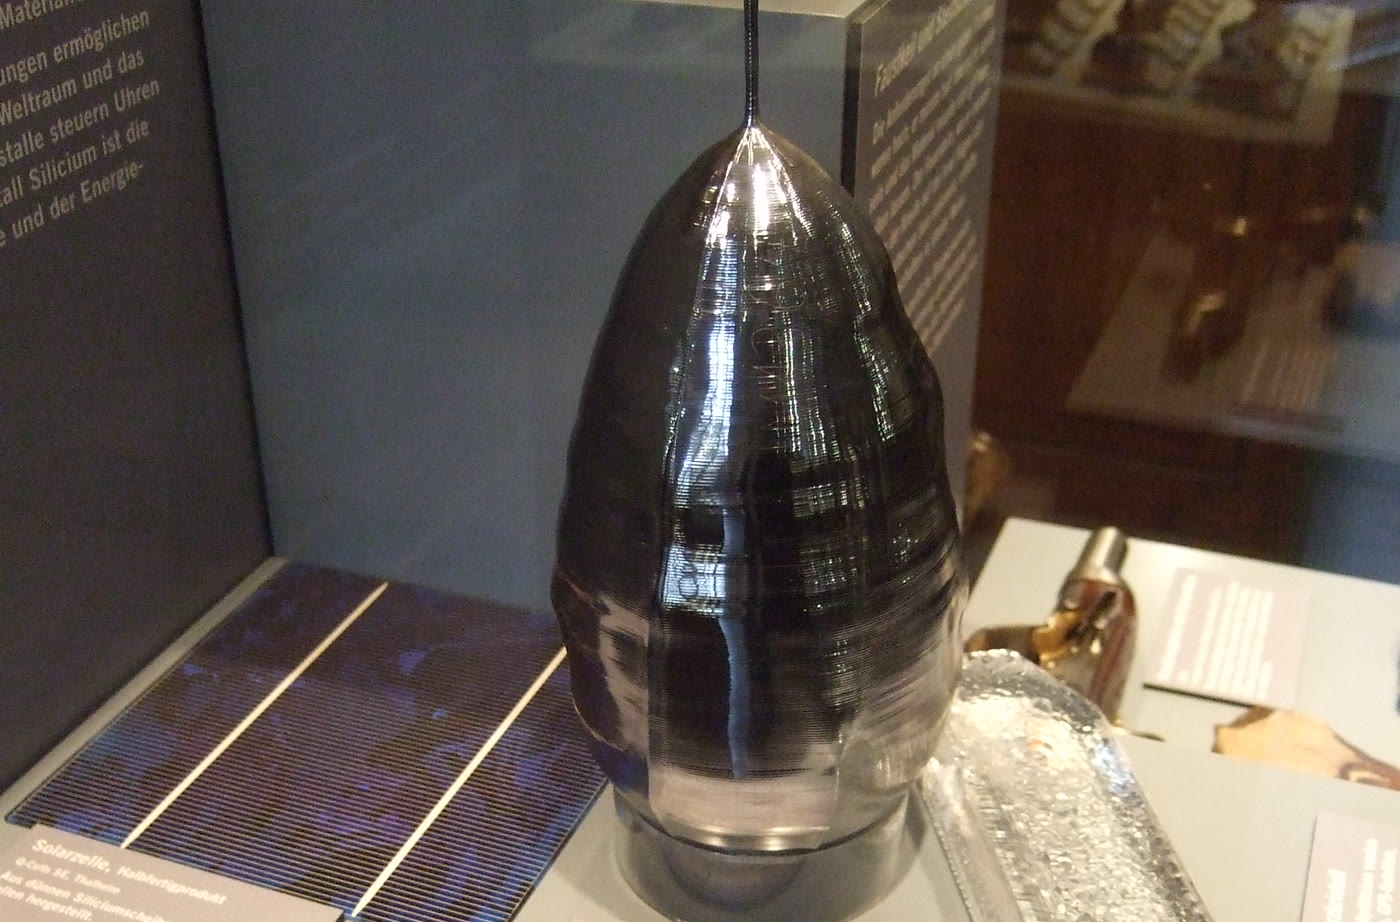
\includegraphics[width=0.5\linewidth]{images/book4/silicon-boule.jpg}

{\small गलित से खींचा गया सिलिकॉन का एक एकल क्रिस्टल, ऐसे क्रिस्टल की एक परत से बने
सौर सेल के बगल में। छायाचित्र: सेबास्टियन वॉलरोथ,
सार्वजनिक अधिकार-क्षेत्र।}
\end{omfigure}

\begin{inthelab}[सिलिकॉन क्रिस्टल उगाना]
चोख्राल्स्की विधि में अति शुद्ध बहुक्रिस्टलीय सिलिकॉन को आर्गन के अधीन सिलिका की
घरिया में, उसके गलनांक से थोड़ा ऊपर, पिघलाया जाता है, और
\omterm{def:b3:solid-state:doping}{अपमिश्रक} को गलित में मिलाया जाता है। घूमती छड़ पर लगे एक छोटे बीज क्रिस्टल को
गलित में डुबोकर धीरे-धीरे ऊपर उठाया जाता है: सिलिकॉन उस पर बीज के
अभिविन्यास के साथ क्रिस्टलित होता है, और खींचने तथा घुमाने की दर व्यास तय करती है। इस
सिल्ली को फिर एक मिलीमीटर से कम मोटी वेफ़रों में काटा जाता है। बाद के चरणों में प्रयुक्त सिलेन और
अपमिश्रण गैसें फ़ॉस्फ़ीन और आर्सीन स्वतःज्वलनशील या अत्यधिक विषैली हैं,
और केवल सीलबंद औद्योगिक प्रणालियों में ही सँभाली जाती हैं।
\end{inthelab}

\section{बिंदु दोष}

\begin{definition}[बिंदु दोष]\label{def:b3:solid-state:defects}
\emph{बिंदु दोष}\index{बिंदु दोष} पूर्ण क्रिस्टल से एक स्थल पर
स्थानीकृत विचलन है: एक रिक्ति, एक अंतराकाशी परमाणु, या एक बाहरी
परमाणु। आयनिक क्रिस्टल में \emph{शॉट्की दोष}\index{शॉट्की दोष}
रिक्तियों का एक युग्म है, एक धनायन और एक ऋणायन, जिनके आयन
पृष्ठ पर चले गए हैं; \emph{फ़्रेंकेल दोष}\index{फ़्रेंकेल दोष} एक
रिक्ति और उसे छोड़ने वाले आयन का युग्म है, जो एक अंतराकाशी स्थल पर बैठा है।
\end{definition}

\begin{omfigure}
\begin{tikzpicture}[scale=0.62]
  \begin{scope}
  \foreach \i in {0,...,5} \foreach \j in {0,...,4} {
    \pgfmathtruncatemacro{\pty}{mod(\i+\j,2)}
    \ifnum\pty=0 \fill[omDef!70] (\i,\j) circle (0.2); \else \fill[omThm!25] (\i,\j) circle (0.38); \draw[omThm!60] (\i,\j) circle (0.38); \fi
  }
  \fill[white] (2,2) circle (0.45); \draw[dashed] (2,2) circle (0.3);
  \fill[white] (3,2) circle (0.45); \draw[dashed] (3,2) circle (0.38);
  \node[font=\small\bfseries] at (2.5,5.0) {शॉट्की (NaCl)};
  \end{scope}
  \begin{scope}[xshift=8cm]
  \foreach \i in {0,...,5} \foreach \j in {0,...,4} {
    \pgfmathtruncatemacro{\pty}{mod(\i+\j,2)}
    \ifnum\pty=0 \fill[black!45] (\i,\j) circle (0.2); \else \fill[omMeth!25] (\i,\j) circle (0.38); \draw[omMeth!60] (\i,\j) circle (0.38); \fi
  }
  \fill[white] (2,2) circle (0.3); \draw[dashed] (2,2) circle (0.22);
  \fill[black!45] (2.5,2.5) circle (0.2);
  \draw[->, thick] (2.1,2.1) -- (2.38,2.38);
  \node[font=\small\bfseries] at (2.5,5.0) {फ़्रेंकेल (AgCl)};
  \end{scope}
\end{tikzpicture}

{\small सैंधव-लवण क्रिस्टल की एक परत में \omterm{def:b3:solid-state:defects}{बिंदु दोष} (छोटे बिंदु: धनायन;
बड़े वृत्त: ऋणायन; धराशायी: रिक्तियाँ)। बाएँ: एक शॉट्की युग्म, एक धनायन
और एक ऋणायन लुप्त। दाएँ: एक फ़्रेंकेल युग्म, एक सिल्वर आयन अपने स्थल से
एक अंतराकाशी स्थिति में खिसका हुआ।}
\end{omfigure}

\begin{theorem}[शॉट्की दोषों की साम्य सांद्रता]\label{thm:b3:solid-state:schottky}
$N$ सूत्र इकाइयों वाले क्रिस्टल MX में साम्य पर शॉट्की युग्मों की संख्या $n$,
प्रति युग्म संभवन एन्थैल्पी $\Delta H_S$ और $n \ll N$ के साथ, है
\[
  \frac{n}{N} = \eu^{-\Delta H_S/2kT}.
\]
\end{theorem}

\begin{proof}
$n$ युग्म बनाने में $n\,\Delta H_S$ लगता है और एक विन्यासी एन्ट्रॉपी मिलती है, जो धनायन रिक्तियाँ चुनने के
$\binom{N}{n}$ प्रकारों से और उतने ही ऋणायनों के लिए आती है:
$S = 2k\ln\frac{N!}{n!(N - n)!}$। स्टर्लिंग सूत्र $\ln x! \approx x\ln x - x$ से,
\[
  G(n) = n\,\Delta H_S - 2kT\bigl[N\ln N - n\ln n - (N - n)\ln(N - n)\bigr].
\]
साम्य पर $\dd G/\dd n = 0$: $\Delta H_S - 2kT\ln\frac{N - n}{n} = 0$, अतः $n/(N - n) = \eu^{-\Delta H_S/2kT}$, और $n/N$,
$n \ll N$ के लिए। दोषों की कंपनिक एन्ट्रॉपी, जिसकी यहाँ उपेक्षा की गई है,
परिणाम को एक नियत गुणक से गुणा करती है।
\end{proof}

\begin{proposition}[फ़्रेंकेल दोष]\label{prop:b3:solid-state:frenkel}
गतिशील प्रकार के $N$ आयनों, उनके लिए उपलब्ध $N_i$ अंतराकाशी स्थलों और
एक युग्म की संभवन एन्थैल्पी $\Delta H_F$ के साथ, फ़्रेंकेल युग्मों की संख्या $n =
\sqrt{NN_i}\,\eu^{-\Delta H_F/2kT}$ है ($n \ll N, N_i$ के लिए)।
\end{proposition}

\begin{proof}
एन्ट्रॉपी अब $S = k\ln\binom{N}{n} + k\ln\binom{N_i}{n}$ है, और वही न्यूनीकरण देता है
\[
  \Delta H_F = kT\ln\frac{(N - n)(N_i - n)}{n^2} \approx kT\ln\frac{NN_i}{n^2},
\]
अतः परिणाम।
\end{proof}

वर्गमूल दिखाता है कि दोष युग्मों में बनते हैं: \omterm{def:b3:solid-state:classes}{अर्धचालक} में $n_i$ की तरह,
उनकी सांद्रता के घातांक में संभवन ऊर्जा का आधा होता है। क्षार
हैलाइड मुख्यतः \omterm{def:b3:solid-state:defects}{शॉट्की दोष} बनाते हैं; सिल्वर हैलाइड, जिनका छोटा, ध्रुवणीय
$\ce{Ag+}$ ऋणायनों के बीच समा जाता है, मुख्यतः \omterm{def:b3:solid-state:defects}{फ़्रेंकेल दोष}।

\begin{definition}[क्रोगर--विंक संकेतन]\label{def:b3:solid-state:kroger-vink}
\emph{क्रोगर--विंक संकेतन}\index{क्रोगर--विंक संकेतन} किसी \omterm{def:b3:solid-state:defects}{बिंदु दोष} को
$\mathrm{A_S^c}$ के रूप में लिखता है: A स्थल पर स्थित स्पीशीज़ है (रिक्ति के लिए V, अंतराकाशी के लिए
स्थल के रूप में $i$), S वह स्थल जिसे वह पूर्ण क्रिस्टल में अधिकृत करती है, और c उस स्थल के सापेक्ष
उसका आवेश: प्रत्येक धनात्मक इकाई के लिए $\bullet$, प्रत्येक ऋणात्मक
इकाई के लिए $'$, किसी के न होने पर $\times$।
\end{definition}

इस प्रकार $\mathrm{V_{Na}'}$ एक सोडियम रिक्ति है (लुप्त $+1$ आपेक्षिक आवेश $-1$ छोड़ता है),
$\mathrm{V_{Cl}^{\bullet}}$ एक क्लोराइड रिक्ति, $\mathrm{Ag_i^{\bullet}}$ एक अंतराकाशी सिल्वर आयन, $\mathrm{Ca_{Na}^{\bullet}}$
सोडियम स्थल पर एक कैल्सियम आयन, $\mathrm{O_O^{\times}}$ अपने स्थान पर एक ऑक्साइड आयन। NaCl का शॉट्की साम्य
$\text{शून्य} \rightleftharpoons \mathrm{V_{Na}' + V_{Cl}^{\bullet}}$ है, AgCl का फ़्रेंकेल साम्य
$\mathrm{Ag_{Ag}^{\times}} \rightleftharpoons \mathrm{Ag_i^{\bullet} + V_{Ag}'}$।

\begin{method}[दोष समीकरण लिखना]\label{met:b3:solid-state:kroger-vink}
\begin{enumerate}
  \item लिखिए कि परपोषी में क्या मिलाया गया और वह कौन-से दोष बनाता है।
  \item स्थल संतुलन: परपोषी के धनायन और ऋणायन स्थलों का अनुपात बना रहता है
        (रिक्तियाँ स्थलों के रूप में गिनी जाती हैं)।
  \item द्रव्यमान संतुलन: दोनों ओर वही परमाणु (रिक्तियों का कोई द्रव्यमान नहीं;
        इलेक्ट्रॉनों $e'$ और \omterm{def:b3:solid-state:carriers}{कोटरों} $h^\bullet$ का भी नहीं)।
  \item आवेश संतुलन: प्रभावी आवेशों के योग बराबर हैं।
\end{enumerate}
\end{method}

\begin{example}[ज़र्कोनिया में यिट्रिया]
$\ce{Y2O3}$ को $\ce{ZrO2}$ में घोलने से दो $\ce{Y^3+}$, $\ce{Zr^4+}$ स्थलों पर आते हैं, प्रत्येक का आपेक्षिक आवेश $-1$, और
तीन ऑक्साइड आयन ऑक्सीजन स्थलों पर; परपोषी के एक धनायन पर दो ऑक्सीजन
स्थलों के अनुपात के लिए दो धनायनों हेतु चार ऑक्सीजन स्थल चाहिए, अतः एक रिक्त रहता है:
\[
  \ce{Y2O3} \xrightarrow{\ce{ZrO2}} \mathrm{2\,Y_{Zr}' + 3\,O_O^{\times} + V_O^{\bullet\bullet}}.
\]
स्थल: 2 धनायन, 4 ऑक्सीजन; द्रव्यमान: 2 Y और 3 O; आवेश: $2(-1) + 2 = 0$। प्रत्येक दो
यिट्रियम आयनों पर एक ऑक्साइड रिक्ति: यही यिट्रिया-स्थायीकृत ज़र्कोनिया को
एक ऑक्साइड-आयन चालक बनाता है।
\end{example}

\begin{definition}[वर्ण केंद्र]\label{def:b3:solid-state:colour-centre}
\emph{वर्ण केंद्र}\index{वर्ण केंद्र} ऐसा \omterm{def:b3:solid-state:defects}{बिंदु दोष} है जो
दृश्य प्रकाश अवशोषित करता है, जैसे किसी क्षार हैलाइड की ऋणायन रिक्ति में फँसा एक इलेक्ट्रॉन
(एक F केंद्र), जो अन्यथा पारदर्शी क्रिस्टल को रंगीन कर देता है।
\end{definition}

सोडियम क्लोराइड को सोडियम वाष्प में गर्म करने या उसे विकिरित करने से F केंद्र बनते हैं:
फँसा इलेक्ट्रॉन रिक्ति के आकार के \omterm{def:b3:quantum-model-systems:box}{डिब्बे में कण} की तरह व्यवहार करता है, और
दृश्य में अवशोषित करता है, जिससे क्रिस्टल पीला-भूरा हो जाता है।

\section{अरससमीकरणमितीयता}

\begin{definition}[अरससमीकरणमितीय यौगिक]\label{def:b3:solid-state:non-stoichiometric}
\emph{अरससमीकरणमितीय यौगिक}\index{अरससमीकरणमितीय यौगिक} वह
ठोस है जिसका संघटन पूर्ण संख्याओं के किसी सरल अनुपात के आसपास एक परास में
बदलता है, और अंतर \omterm{def:b3:solid-state:defects}{बिंदु दोषों} द्वारा समायोजित होता है।
\end{definition}

आयरन(II) ऑक्साइड कभी भी ठीक $\ce{FeO}$ नहीं होता: उसमें सदैव आयरन की कमी होती है,
$\mathrm{Fe_{1-x}O}$, जहाँ $x$ उस ताप और ऑक्सीजन दाब से तय होता है जिस पर वह बनाया गया। प्रत्येक लुप्त $\ce{Fe^2+}$ की क्षतिपूर्ति दो
$\ce{Fe^3+}$ करते हैं, जो दोष की भाषा में आयरन स्थलों पर \omterm{def:b3:solid-state:carriers}{कोटर} हैं।

\begin{proposition}[चालकता और ऑक्सीजन दाब]\label{prop:b3:solid-state:brouwer}
धातु-न्यून ऑक्साइड $\mathrm{M_{1-x}O}$ के लिए, जिसके दोष \omterm{def:b3:solid-state:carriers}{कोटरों} द्वारा क्षतिपूरित द्वि-आवेशित धातु रिक्तियाँ हैं,
\omterm{def:b3:solid-state:carriers}{कोटर} सांद्रता, और चालकता,
$p(\ce{O2})^{1/6}$ के अनुसार बदलती हैं। इलेक्ट्रॉनों द्वारा क्षतिपूरित ऑक्सीजन-न्यून ऑक्साइड के लिए वे
$p(\ce{O2})^{-1/6}$ के अनुसार बदलती हैं।
\end{proposition}

\begin{proof}
ऑक्सीजन ग्रहण करने से धातु रिक्तियाँ बनती हैं:
\[
  \tfrac12\ce{O2} \rightleftharpoons \mathrm{O_O^{\times} + V_M'' + 2\,h^{\bullet}}, \qquad K = \frac{[\mathrm{V_M''}][\mathrm h^\bullet]^2}{p(\ce{O2})^{1/2}}
\]
($\mathrm{O_O^{\times}}$ की सक्रियता 1 है)।
आवेश संतुलन $[\mathrm h^\bullet] = 2[\mathrm{V_M''}]$ है, अतः $[\mathrm h^\bullet]^3 = 2K\,p(\ce{O2})^{1/2}$ और $[\mathrm h^\bullet] \propto p(\ce{O2})^{1/6}$।
ऑक्सीजन-न्यून स्थिति के लिए $\mathrm{O_O^{\times}} \rightleftharpoons \tfrac12\ce{O2} + \mathrm{V_O^{\bullet\bullet} + 2\,e'}$, $[\mathrm e'] = 2[\mathrm{V_O^{\bullet\bullet}}]$, और वही चरण $[\mathrm e'] \propto p(\ce{O2})^{-1/6}$ देते हैं।
चालकता वाहक सांद्रता के समानुपाती है।
\end{proof}

इस प्रकार $\log\sigma$ का $\log p(\ce{O2})$ के विरुद्ध आलेख बताता है कि कौन-से दोष प्रभावी हैं: उसका ढलान,
$\pm 1/4$ या $\pm 1/6$, उनके आवेशों पर निर्भर करता है।

\section{आयनिक चालक}

\begin{definition}[आयनिक चालक]\label{def:b3:solid-state:ionic-conductor}
\emph{आयनिक चालक}\index{आयनिक चालक} वह ठोस है जिसमें धारा
जालक से होकर गति करते आयनों द्वारा वहन की जाती है। \emph{ठोस
विद्युत-अपघट्य}\index{ठोस विद्युत-अपघट्य} वह आयनिक चालक है जिसकी इलेक्ट्रॉनिक
चालकता नगण्य हो, ताकि वह किसी विद्युतरासायनिक सेल के दोनों इलेक्ट्रोडों को
पृथक कर सके।
\end{definition}

\begin{proposition}[आयनिक चालन का आरेनियस नियम]\label{prop:b3:solid-state:ionic-arrhenius}
अवरोध $E_a$ के ऊपर से पड़ोसी स्थलों के बीच कूदकर गति करने वाले आयनों के लिए,
$\sigma T = A\,\eu^{-E_a/kT}$।
\end{proposition}

\begin{proof}[आंशिक उपपत्ति]
एक आयन आवृत्ति $\nu_0$ पर छलाँग का प्रयास करता है और प्रायिकता $\eu^{-E_a/kT}$ के साथ सफल होता है,
अतः उसका विसरण गुणांक $D = \tfrac16\nu_0 z a^2\eu^{-E_a/kT}$ है, $z$ पड़ोसी स्थलों के लिए, जो
दूरी $a$ पर हैं (यादृच्छिक भ्रमण)। नेर्न्स्ट--आइंस्टाइन संबंध $\sigma = nq^2D/kT$ (स्वीकृत), $n$
गतिशील आयनों के लिए जिनका आवेश $q$ है, प्रति इकाई आयतन, $\sigma T = (nq^2\nu_0za^2/6k)\,\eu^{-E_a/kT}$ देता है।
बाह्य चालक में सांद्रता $n$ अपमिश्रण द्वारा नियत होती है; जब वह
स्वयं तापीय रूप से बनती है, तो $E_a$ में संभवन एन्थैल्पी का आधा भी सम्मिलित होता है।
\end{proof}

% ledger: trans:AgI
तीन \omterm{def:b3:solid-state:ionic-conductor}{ठोस विद्युत-अपघट्य} इस परास को दिखाते हैं। यिट्रिया-स्थायीकृत ज़र्कोनिया में
\omterm{def:b3:solid-state:doping}{अपमिश्रक} द्वारा बनी ऑक्साइड रिक्तियाँ $\ce{O^2-}$ आयनों को कूदने देती हैं; यह केवल गर्म होने पर,
कई सौ डिग्री सेल्सियस पर, उपयोगी चालन करता है। $\beta$-ऐलुमिना में सोडियम आयन
स्पिनेल खंडों के बीच ढीले संकुलित तलों में गति करते हैं, जो सोडियम--सल्फ़र
बैटरियों का आधार है। सिल्वर आयोडाइड \qty{146}{\celsius} से ऊपर एक अति-आयनिक चालक बन जाता है,
जहाँ उसके सिल्वर आयन आयनों की संख्या से कहीं अधिक स्थलों पर फैले होते हैं,
एक दृढ़ आयोडाइड जालक के भीतर लगभग द्रव की तरह। लिथियम-आयन चालक
(लिथियम लैंथेनम ज़र्कोनेट गार्नेट, सल्फ़ाइड) अब विकसित हो रही
पूर्ण-ठोस बैटरियों के विद्युत-अपघट्य हैं।

\begin{omfigure}
\begin{tikzpicture}[font=\small, >=Stealth]
  \fill[omProp!25] (0,0) rectangle (2.4,3.2);
  \node[font=\scriptsize, align=center] at (1.2,0.6) {$\ce{ZrO2}$--$\ce{Y2O3}$\\ ठोस विद्युत-अपघट्य};
  \draw[black!60, line width=2.5pt] (-0.07,0) -- (-0.07,3.2);
  \draw[black!60, line width=2.5pt] (2.47,0) -- (2.47,3.2);
  \node[font=\scriptsize, align=center] at (-2.0,1.4) {निकास गैस\\ $p(\ce{O2})$ कम};
  \node[font=\scriptsize, align=center] at (4.4,1.4) {संदर्भ वायु\\ $p(\ce{O2}) = \qty{0.21}{bar}$};
  \node[font=\scriptsize, anchor=north] at (-0.07,-0.05) {Pt};
  \node[font=\scriptsize, anchor=north] at (2.47,-0.05) {Pt};
  \draw[->, thick, omThm] (2.0,1.9) -- (0.4,1.9) node[midway, above, font=\scriptsize] {$\ce{O^2-}$};
  \node[font=\scriptsize, anchor=west] at (2.65,2.75) {$\ce{O2 + 4e- -> 2O^2-}$};
  \node[font=\scriptsize, anchor=east] at (-0.25,2.75) {$\ce{2O^2- -> O2 + 4e-}$};
  \draw (-0.07,3.2) -- (-0.07,4.0) -- (0.85,4.0);
  \draw (2.47,3.2) -- (2.47,4.0) -- (1.55,4.0);
  \draw (1.2,4.0) circle (0.35) node {V};
\end{tikzpicture}

{\small अनुप्रस्थ काट में ज़र्कोनिया ऑक्सीजन संवेदक: \omterm{def:b3:solid-state:ionic-conductor}{ठोस विद्युत-अपघट्य} के
दोनों फलकों पर सरंध्र प्लैटिनम इलेक्ट्रोड, एक निकास में और एक वायु में।
ऑक्साइड आयन विद्युत-अपघट्य से होकर धारा वहन करते हैं; वोल्टता
दोनों ऑक्सीजन दाबों का अनुपात मापती है।}
\end{omfigure}

\begin{history}[ट्रांज़िस्टर और खींचा गया क्रिस्टल]
1947 में जॉन बार्डीन और वॉल्टर ब्रैटेन ने, बेल
प्रयोगशालाओं में विलियम शॉक्ली के समूह में, जर्मेनियम के एक क्रिस्टल से पहला ट्रांज़िस्टर बनाया; तीनों ने
भौतिकी का 1956 का नोबेल पुरस्कार साझा किया। क्रिस्टल यान
चोख्राल्स्की की 1916 में खोजी गई एक विधि से आए थे, जो उन्होंने यह मापते हुए पाई थी कि धातुएँ कितनी तेज़ी से क्रिस्टलित होती हैं,
गलित से टिन का एक धागा खींचकर: जर्मेनियम और फिर सिलिकॉन के लिए अनुकूलित होकर,
यह आज भी लगभग सभी एकीकृत परिपथों के वेफ़र बनाती है।
\end{history}

\section{अभ्यास}

\begin{exercise}[$\star$]\label{exo:b3:solid-state:1}
छह परमाणुओं की शृंखला के छह ह्युकेल स्तर $|\beta|$ की इकाइयों में, और उनके द्वारा घेरे गए परास
की चौड़ाई बताइए।
\end{exercise}

\begin{exercise}[$\star$]\label{exo:b3:solid-state:2}
$N$ परमाणुओं के s कक्षकों से बना बैंड कितने इलेक्ट्रॉन रखता है? सोडियम और मैग्नीशियम
दोनों धातु क्यों हैं?
\end{exercise}

\begin{exercise}[$\star$]\label{exo:b3:solid-state:3}
$\lambda \approx hc/E_g$ का उपयोग करके गैलियम फ़ॉस्फ़ाइड
(\qty{2.26}{eV}) और गैलियम नाइट्राइड (\qty{3.4}{eV}) के डायोडों द्वारा उत्सर्जित प्रकाश की तरंगदैर्ध्य का आकलन कीजिए।
\end{exercise}

\begin{exercise}[$\star$]\label{exo:b3:solid-state:4}
$\ce{CaCl2}$ को $\ce{NaCl}$ में और $\ce{Y2O3}$ को $\ce{ZrO2}$ में घोलने के लिए क्रोगर--विंक समीकरण लिखिए, और
प्रत्येक संतुलन जाँचिए।
\end{exercise}

\begin{exercise}[$\star\star$]\label{exo:b3:solid-state:5}
सिलिकॉन के लिए \qty{300}{K} पर $N_c = \num{6.2e15}\,T^{3/2}$, $N_v = \num{3.5e15}\,T^{3/2}$ ($\unit{cm^{-3}}$ में) और $E_g = \qty{1.125}{eV}$ के साथ,
तथा जर्मेनियम के लिए $N_c = \num{1.98e15}\,T^{3/2}$, $N_v = \num{9.6e14}\,T^{3/2}$, $E_g = \qty{0.661}{eV}$ के साथ, प्रत्येक के लिए $n_i$, और उनका
अनुपात, परिकलित कीजिए।
\end{exercise}

\begin{exercise}[$\star\star$]\label{exo:b3:solid-state:6}
सिलिकॉन को $\qty{1.0e16}{cm^{-3}}$ फ़ॉस्फ़ोरस से अपमिश्रित किया गया है। \qty{300}{K} पर $n_i = \qty{1.0e10}{cm^{-3}}$ के साथ,
इलेक्ट्रॉन और \omterm{def:b3:solid-state:carriers}{कोटर} सांद्रताएँ बताइए।
\end{exercise}

\begin{exercise}[$\star\star$]\label{exo:b3:solid-state:7}
\cref{exo:b3:solid-state:6} के क्रिस्टल के लिए \omterm{def:b3:solid-state:fermi}{फ़र्मी स्तर} नैज स्तर से
कितना ऊपर है?
\end{exercise}

\begin{exercise}[$\star\star$]\label{exo:b3:solid-state:8}
NaCl में शॉट्की युग्म की संभवन एन्थैल्पी लगभग \qty{2.3}{eV} है (अभ्यास के
आँकड़े)। \qty{800}{K} पर रिक्त स्थलों का अंश, और एक मोल में
युग्मों की संख्या परिकलित कीजिए।
\end{exercise}

\begin{exercise}[$\star\star$]\label{exo:b3:solid-state:9}
आयरन(II) ऑक्साइड के एक नमूने (सैंधव-लवण संरचना, प्रति कोष्ठिका चार ऑक्सीजन स्थल) के लिए
$a = \qty{430.0}{pm}$ और घनत्व \qty{5.70}{g.cm^{-3}} है (अभ्यास के आँकड़े)। ऑक्सीजन स्थलों को
पूरा भरा मानकर $x$ ज्ञात कीजिए, $\mathrm{Fe_{1-x}O}$ में।
\end{exercise}

\begin{exercise}[$\star\star\star$]\label{exo:b3:solid-state:10}
एक लिथियम-आयन चालक के लिए \qty{300}{K} पर $\sigma = \qty{1.0e-4}{S.cm^{-1}}$, \qty{350}{K} पर $\qty{7.8e-4}{S.cm^{-1}}$ और
\qty{400}{K} पर $\qty{3.6e-3}{S.cm^{-1}}$ है (अभ्यास के आँकड़े)। इसकी सक्रियण ऊर्जा ज्ञात कीजिए।
\end{exercise}

\begin{exercise}[$\star\star\star$]\label{exo:b3:solid-state:11}
दिखाइए कि जिस ऑक्साइड के प्रभावी दोष \omterm{def:b3:solid-state:carriers}{कोटरों} द्वारा क्षतिपूरित एकल-आवेशित धातु रिक्तियाँ
$\mathrm{V_M'}$ हों, उसमें चालकता $p(\ce{O2})^{1/4}$ के अनुसार बदलती है।
\end{exercise}

\begin{exercise}[$\star\star\star$]\label{exo:b3:solid-state:12}
AgCl में फ़्रेंकेल युग्म की संभवन एन्थैल्पी लगभग \qty{1.4}{eV} है, और प्रति सिल्वर आयन
दो अंतराकाशी स्थल हैं (अभ्यास के आँकड़े)। \qty{600}{K} पर अंतराकाशी स्थलों पर स्थित
सिल्वर आयनों का अंश परिकलित कीजिए।
\end{exercise}

\section{समस्या: निकास नली में ऑक्सीजन संवेदक}

\begin{problem}[{सप्ताहांत समस्या --- निकास नली में ऑक्सीजन संवेदक:
यिट्रिया-स्थायीकृत ज़र्कोनिया के दोष, उसकी आयनिक चालकता और प्रचालन
ताप, सेल की नेर्न्स्ट वोल्टता, और विरल तथा
समृद्ध निकास के बीच स्विच}]
\label{pb:b3:solid-state:1}
% ledger: const:R, const:F, const:kB, const:e, const:NA, air:O2
संवेदक का विद्युत-अपघट्य 8.0\,mol\,\% $\ce{Y2O3}$ वाला ज़र्कोनिया है, फ़्लुओराइट संरचना का,
प्रति घनीय कोष्ठिका चार धनायन और आठ ऑक्सीजन स्थलों के साथ, $a = \qty{514}{pm}$; \qty{1.0}{mm}
मोटी और \qty{0.20}{cm^2} क्षेत्रफल की एक चकती निकास को वायु से अलग करती है। इसकी
चालकता $\sigma T = A\eu^{-E_a/kT}$ का पालन करती है, जहाँ $E_a = \qty{1.0}{eV}$ और \qty{800}{\celsius} पर $\sigma = \qty{0.030}{S.cm^{-1}}$। विरल
निकास में $p(\ce{O2}) = \qty{0.010}{bar}$, समृद्ध निकास में $p(\ce{O2}) = \qty{1.0e-20}{bar}$ (सभी आँकड़े समस्या के)।

\medskip\noindent\textbf{भाग I --- विद्युत-अपघट्य।}
\begin{enumerate}
  \item $\ce{Y2O3}$ को $\ce{ZrO2}$ में घोलने का क्रोगर--विंक समीकरण लिखिए।
  \item इसका स्थल, द्रव्यमान और आवेश संतुलन जाँचिए।
  \item प्रति यिट्रियम आयन कितनी ऑक्साइड रिक्तियाँ बनती हैं?
  \item संघटन को $\mathrm{Zr_{1-x}Y_xO_{2-x/2}}$ के रूप में लिखिए और $x$ परिकलित कीजिए।
  \item रिक्त ऑक्सीजन स्थलों का अंश परिकलित कीजिए।
  \item प्रति कोष्ठिका रिक्तियों की संख्या परिकलित कीजिए।
  \item रिक्ति सांद्रता $\unit{cm^{-3}}$ में परिकलित कीजिए।
\end{enumerate}

\medskip\noindent\textbf{भाग II --- चालकता और ताप।}
\begin{enumerate}[resume]
  \item ताप के साथ चालकता तेज़ी से क्यों बढ़ती है?
  \item $A$ परिकलित कीजिए।
  \item \qty{700}{\celsius} पर $\sigma$ परिकलित कीजिए।
  \item \qty{300}{\celsius} पर $\sigma$ परिकलित कीजिए।
  \item इन दोनों तापों पर चकती का प्रतिरोध परिकलित कीजिए।
  \item इलेक्ट्रॉनिकी को \qty{1}{k\ohm} से कम प्रतिरोध चाहिए: न्यूनतम प्रचालन
        ताप ज्ञात कीजिए।
  \item ऐसे संवेदकों में तापक क्यों लगाया जाता है?
\end{enumerate}

\medskip\noindent\textbf{भाग III --- नेर्न्स्ट वोल्टता।}
\begin{enumerate}[resume]
  \item वायु वाले पक्ष की इलेक्ट्रोड अभिक्रिया सामान्य और
        \omterm{def:b3:solid-state:kroger-vink}{क्रोगर--विंक संकेतन} में लिखिए।
  \item दिखाइए कि सेल वोल्टता $E = (RT/4F)\ln\bigl(p_{\text{वायु}}/p_{\text{निकास}}\bigr)$ है।
  \item \qty{700}{\celsius} पर $RT/4F$ परिकलित कीजिए।
  \item यदि निकास में वायु होती तो वोल्टता क्या होती?
  \item $p(\ce{O2})$ में दस गुना परिवर्तन पर वोल्टता का परिवर्तन परिकलित कीजिए।
\end{enumerate}

\medskip\noindent\textbf{भाग IV --- विरल, समृद्ध और स्विच।}
\begin{enumerate}[resume]
  \item \qty{700}{\celsius} पर विरल निकास में वोल्टता परिकलित कीजिए।
  \item \qty{700}{\celsius} पर समृद्ध निकास में वोल्टता परिकलित कीजिए।
  \item समृद्ध निकास में $p(\ce{O2})$ इतना छोटा क्यों है?
  \item इंजन नियंत्रण \qty{0.45}{V} पर स्विच करता है: यह किस ऑक्सीजन दाब के
        संगत है?
  \item रससमीकरणमितीय वायु-से-ईंधन अनुपात पर वोल्टता उछलती क्यों है, और इंजन नियंत्रण
        इसका उपयोग कैसे करता है?
  \item परिणाम बताइए: \qty{700}{\celsius} पर समृद्ध निकास में संवेदक वोल्टता।
\end{enumerate}
\end{problem}
